\documentclass[main]{subfiles}
\begin{document}

\section{先行実装}
\subsection{データセット}
評価用データセットとしてDomestic Environment Sound Event Detection Dataset (DESED)，
および MAESTRO Real の21クラスを使用する\cite{turpault2019sound,serizel2020sound,martin2023strong}．\par

これらデータセットのラベルには種類がある．弱ラベルはイベント種別のみを，強ラベルは開始・終了時刻も含み，それぞれクリップとフレームに対応する．\par

データセットに含まれる音声について，DESEDは家庭内の音響イベント検出に向けて，実環境で録音した家庭内の生活音と，そのような環境を再現するために合成された音が含まれる．
音声データは10秒間のモノラルオーディオで，サンプリングレート 16kHz または 44.1kHzとなっている．
% モノラル > チャネル数が1
MAESTRO Realは実環境の$3-5$分の音が含まれる．ラベルは0か1ではなく，0.8などの連続値 (ソフトラベル) で，強ラベルが付与されている．\par

% そのうち，10（Alarm bell ringing，Blender，Cat，Dishes，Dog，Electric shaver toothbrush，Frying，Running water，Speech，Vacuum cleaner）及び11（Birds singing，Car，People talking，Footsteps，Children voices，Wind blowing，Brakes squeaking，Large vehicle，Cutlery and dishes，Metro approaching，Metro leaving）クラスを使用する．\par
% DESEDのデータは学習の利用段階とデータの作成法，ラベルで分類される．利用段階には訓練，検証，評価がある．データは実環境の録音か，あるいは合成で作成され，ラベルは強，弱，なしに分類される．
% ここで，ラベルの強・弱はフレーム・クリップに対応しており，フレームごとにイベントの開始・終了・種類が記録されていれば強ラベル，10秒のクリップに対して含まれるイベントの種類のみであった場合は弱ラベルに分類される．ラベルなしは全くラベルが付加されていないデータを指す．
% なお，本稿では一部データが取得できず，通常より少ないデータ数で学習を行っている．本稿で使用したDESEDのデータ数は表\ref{table:desed}の通り．\par
% \begin{table}[htbp]
%  \begin{center}
%    \begin{tabular}{|l|c|c|}
%     \hline
%     利用段階 & データ種別  & 数[clips] \\
%     \hline
%     訓練 & 強ラベル，実録音 & 1613 \\
%     訓練 & 弱ラベル，実録音 & 1188 \\
%     訓練 & 強ラベル，合成音 & 10000 \\
%     訓練 & ラベルなし，実録音 & 12027 \\
%     検証 & 弱ラベル，実録音 & 129 \\
%     検証 & 強ラベル，合成音 & 2500 \\
%     評価 & 強ラベル，実録音  & 958 \\
%     \hline
%   \end{tabular}
%   \caption{データ数}
%   \label{table:desed}
% \end{center}
% \end{table}

\subsection{評価指標}
    \label{評価指標}
本稿ではDCASE2024に基づき，データセットに応じて異なる評価指標を採用する．
DESEDではPolyphonic Sound Detection Score（PSDS）\cite{bilen2020framework}のシナリオ1及び2を用い，
MAESTRO RealではmpAUC（Macro-averaged Partial AUC．なお，AUC (Area Under the Curve) はROC (Receiver Operating Characteristic) 曲線の下部）を主要な指標とする．\par

PSDSは，混同行列に基づくROC曲線を拡張したPSD-ROC曲線を用いて算出される．
通常のROC曲線は，縦軸に真陽性率（TPR），横軸に偽陽性率（FPR）をとるが，
PSD-ROC曲線では横軸に単位時間あたりの誤検知数（Effective False Positive Rate）を採用する点が異なる．

PSDSには目的に応じたシナリオが存在する．
シナリオ1（$PSDS_1$）は時間的な正確さを重視し，イベントの検知区間が正解と厳密に一致することを求める一方，クラス分類の誤りには比較的寛容である．
対照的に，シナリオ2（$PSDS_2$）はイベントのクラス分類性能を重視し，時間的なズレに対する許容範囲が広く設定されている．

本稿では，時間精度の向上とイベント分類の最適化を段階的に分離することを想定しており，現段階では正確なクラス分類を優先課題としている．
したがって，$PSDS_2$を最重要指標と位置付けるが，モデルの総合的な挙動を把握するため$PSDS_1$も併せて評価する．\par

一方，MAESTRO Realの評価に用いるmpAUCは，ROC曲線の全領域ではなく，誤検知率が低い領域（低FPR領域）に限定して曲線下面積（AUC）を算出する指標である．
これは，実用上許容できない高い誤検知率の領域を評価から除外することで，モデルの信頼性をより厳密に評価するためである．

\subsection{先行実装モデルの流れ}
先行実装モデルの処理は学習と検証，評価の三段階に区分される．これ以降，先行実装モデルについて，基本的にDCASE 2024の公式設定に準拠する．\par
データの前処理の後，学習を150エポック行う．モデルは入力に対し，ラベルごとの予測（弱/強 予測）を出力する．予測と正解ラベルを用いて教師あり及び半教師あり学習の損失を計算し，Adam\cite{kingma2014adam}で生徒モデルを，指数移動平均で教師モデルを更新する．\par
検証は10エポックごとに行う．学習したモデルで検証用データを入力に推論し，精度を測る．過去の検証時より向上した場合，評価及び推論用に重みパラメータを保持する．評価は評価用データで検証と同様の作業が行われる．\par

\subsection{モデル構成}
\label{DCASE:モデル構成}
\begin{figure}[htbp]
    \centering
    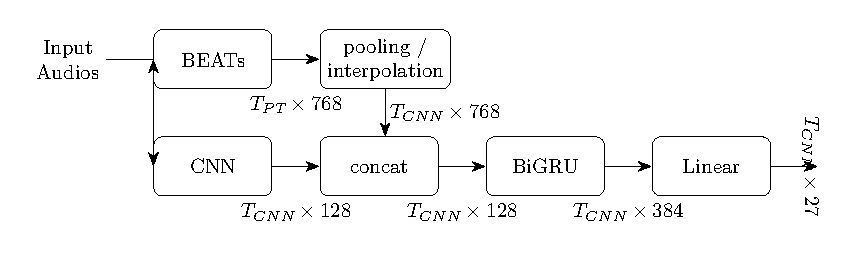
\includegraphics[width=\columnwidth]{figures/model.pdf}
    \caption{各段階の次元数は特徴量の時間長 (フレーム数) と周波数を表す．BEATsの出力を調整してCNNの出力と統合．RNNに入力し，最終的に予測を得る．なお，T: 時間長, PT: 事前学習モデルとする．}
    % 図の説明をより詳細にする．
    \label{fig:model}
\end{figure}

先行実装は図\ref{fig:model}のように，時間周波数領域の局所的な特徴を抽出するCNNと，時系列情報を学習しイベントの時間的変化をモデル化する再帰型ニューラルネットワーク（Recurrent Neural Network; RNN）を組み合わせた，CRNN（Convolutional Recurrent Neural Network）アーキテクチャである．
特徴抽出器として事前学習されたBEATs（Bidirectional Encoder representation from Audio Transformers）\cite{chen2022beats} を用いて，学習コストを抑制しながらタスクに有効な特徴表現を獲得する．\par
BEATsへの入力はCNNと次元数が異なるが，出力は時間解像度を補間することでCNNと統合される．

\subsubsection{CNN}
CNNは7つの畳み込みブロックで構成され，ブロックはConv2D，Batch Normalization，ReLU，Dropout，及びMaxPool2Dを順に積層する．
BEATsの出力との統合のため特徴量の次元数（バッチ数，チャネル数，時間長 (フレーム数) ，周波数）を調整し，RNNに出力する．

% \begin{figure}[htbp]
%     \centering
%     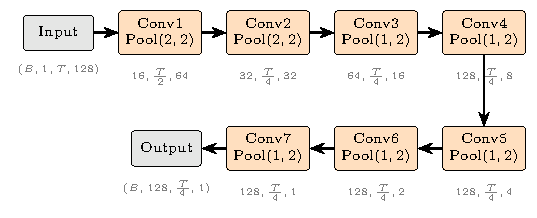
\includegraphics[width=100mm]{figures/cnn_3.pdf}
%     \caption{CNNの構造を示す．畳み込み層を含んだブロックが7つあり，これらは役割に応じて三種類に大別される．各要素の下の数値は特徴量の次元数（バッチ数，チャネル数，時間長 (フレーム数) ，周波数）を表す．}
%     \label{fig:cnn}
% \end{figure}

\subsubsection{RNN}
% (図\ref{fig:rnn}) 
RNNには双方向Gated Recurrent Unit（Bidirectional GRU; BiGRU）を使用し，順方向と逆方向に特徴を処理することで，イベントの時間的な変化を学習する．\par

% \begin{figure}[htbp]
%     \centering
%     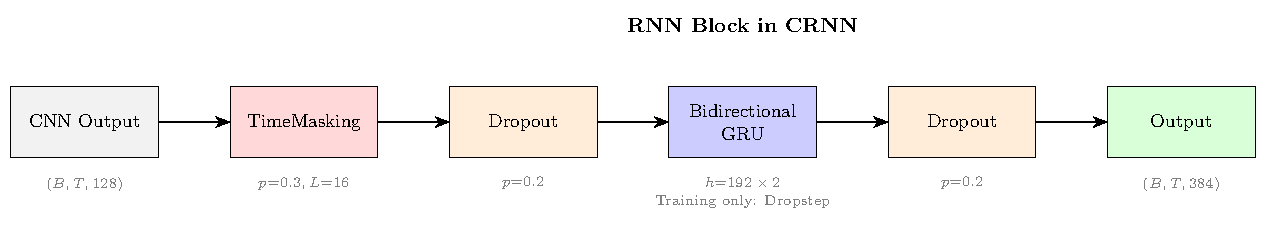
\includegraphics[width=150mm]{figures/rnn_2_horizontal.pdf}
%     \caption{RNNの構造を示す．CNNからの入力を受け取ってTime Masking・Dropoutと順に適用し，BiGRU層に入力した後，再度Dropoutを適用する．なお，図中のhはRNNの隠れ層の数を表す．}
%     \label{fig:rnn}
% \end{figure}

% \subsubsection{予測の出力}
% \begin{figure}[htbp]
%     \centering
%     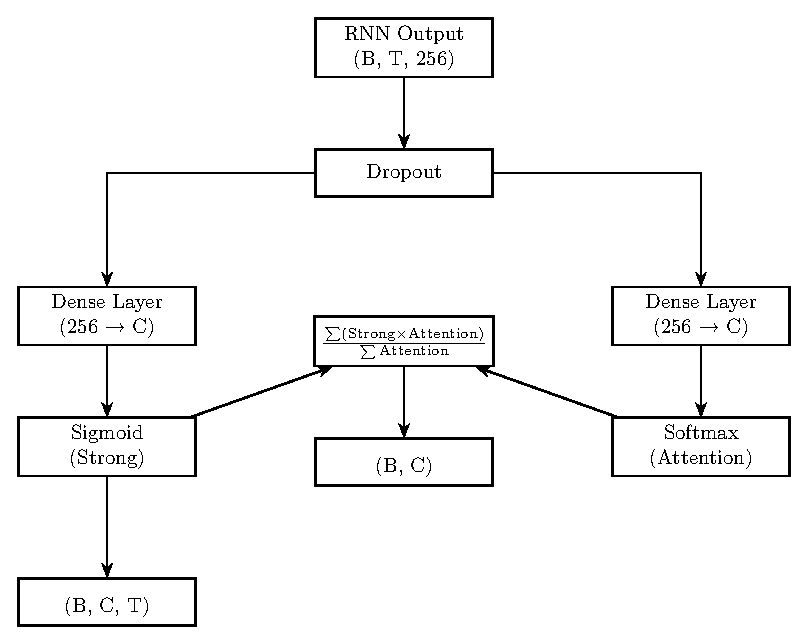
\includegraphics[width=110mm]{figures/linear_2.pdf}
%     \caption{出力の構造を示す．各文字について，B: バッチ数，C: クラス数，T: 時間長（フレーム数）を表す．}
%     \label{fig:linear}
% \end{figure}

\subsection{出力}
先行実装の出力段はRNNの出力（$\text{Batch} \times \text{Time} \times 384$）を強/弱予測に変換する．
出力は全結合層とSigmoid活性化関数で27クラスに対する強予測に変換され，それらをAttention機構による時間方向に集約して弱予測を得る．
なお，評価に用いるのは21クラスである．

\end{document}